\documentclass[12pt,a4paper]{article}

\usepackage[T1,T2A]{fontenc}
\usepackage[utf8]{inputenc}
\usepackage[english, russian]{babel}
\usepackage{indentfirst}
\usepackage{misccorr}
\usepackage{graphicx}
\usepackage{amsmath}
\usepackage{graphicx}
\usepackage{float}
\usepackage[left=20mm,right=10mm, top=20mm,bottom=20mm,bindingoffset=0mm]{geometry}

\setlength{\parskip}{6pt}\graphicspath{{images/}}\DeclareGraphicsExtensions{.png}

\begin{document}

    \begin{titlepage}
        \begin{center}
            \large
            Санкт-Петербургский политехнический университет\\Петра Великого\\
            \vspace{0.5cm}
            Физико-механический институт\\
            \vspace{0.25cm}
            Кафедра «Прикладная математика»
            \vfill
            \textsc{\LARGE\textbf{Отчет по лабораторной работе №1}}\\[5mm]
            \Large
            по дисциплине\\"Математическая статистика"
        \end{center}
        \vfill
        \begin{tabular}{l p{175pt} l}
            Выполнил студент \\ группы 5030102/000101 && Нгуен Хоанг Линь
            \vspace{0.25cm}
            \\Проверил \\ доцент, к.ф.-м.н. && Баженов Александр Николаевич
        \end{tabular}
        \vfill
        \begin{center}
            Санкт-Петербург \\ 2023 г.
        \end{center}
    \end{titlepage}

\newpage
\begin{center}
    \tableofcontents
    \setcounter{page}{2}
\end{center}
\newpage
\begin{center}
    \listoffigures
\end{center}

\newpage
\section{Постановка задачи}
Для 5 распределений:
\begin{itemize}
    \item Нормальное распределение $N(x,0,1)$
    \item Распределение Коши $C(x,0,1)$
    \item Распределение Лапласа $L(x,0,\frac{1}{\sqrt{2}})$
    \item Распределение Пуассона $P(k,10)$
    \item Равномерное распределение $U(x,-\sqrt{3},\sqrt{3})$
\end{itemize}

Необходимо:
\begin{enumerate}
    \item Сгенерировать выборки размером 10, 50 и 1000 элементов
    \item Построить на одном рисунке гистограмму и график плотности распределения
\end{enumerate}

\section{Теория}
\subsection{Рассматриваемые распределения}
Плотности:
\begin{itemize}
		\item Нормальное распределение
		    \begin{equation}
			    N(x,0,1)=\frac{1}{\sqrt{2\pi}}e^{-\frac{x^2}{2}}
			    \label{normal} 
			\end{equation}
		\item Распределение Коши
		    \begin{equation}
				C(x,0,1)=\frac{1}{\pi}\frac{1}{x^2+1}
				\label{cauchy}
			\end{equation} 
		\item Распределение Лапласа
		    \begin{equation}
				L(x,0,\frac{1}{\sqrt{2}})=\frac{1}{\sqrt{2}}e^{-\sqrt{2}|x|}
				\label{laplace} 
			\end{equation}
		\item Распределение Пуассона
		    \begin{equation}
				P(k,10)=\frac{10^k}{k!}e^{-10}
				\label{poisson}
			\end{equation}
		\item Равномерное распределение
		    \begin{equation}
				U(x,-\sqrt{3},\sqrt{3})=
				\begin{cases}
					\frac{1}{2\sqrt{3}},|x|\leq\sqrt{3}\\0,|x|>\sqrt{3}
				\end{cases}
				\label{uniform}
			\end{equation}
\end{itemize}

\subsection{Гистограмма}
\textit{Гистограмма} - графический метод отображения и исследования рядов распределения значения случайной величины. Строится на основе выборки из некоторого распределения и приближает плотность его вероятности.

Построение гистограммы:
\begin{enumerate}
    \item Множество значений, которые может принимать элемент выборки, разбивается на несколько, чаще всего равных, интервалов
    \item Эти интервалы откладываются на горизонтальной оси
    \item Над каждым из интервалов рисуется прямоугольник:
        \begin{itemize}
            \item Если интервалы одинаковы, то высота каждого прямоугольника пропорциональна числу элементов выборки, попадающих в данный интервал
            \item Если интервалы разные, то площадь каждого прямоугольника пропорциональна числу элементов выборки, попадающих в данный интервал 
        \end{itemize}
\end{enumerate}

\section{Реализация}
Лабораторная работа выполнена на языке Python в виртуальной среде Anaconda с интерпретатором версии 3.9 в среде разработки Visual Studio Code. Дополнительные зависимости:
\begin{itemize}
    \item matplotlib
    \item scipy
    \item numpy
\end{itemize}


\section {Результаты}
\begin{figure}[H]
    \centering
    \begin{tabular}{c c c}
        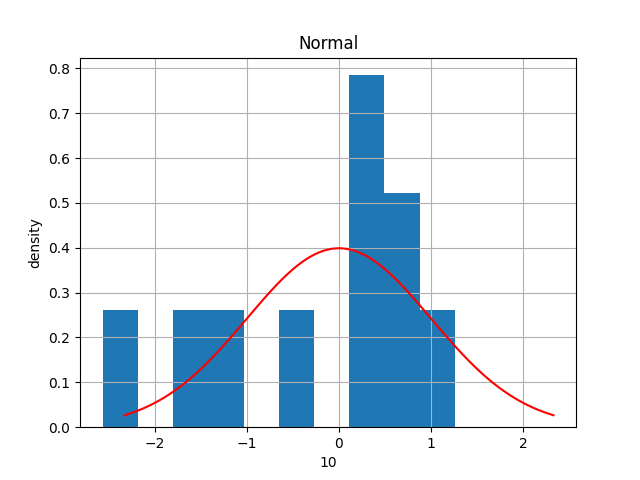
\includegraphics[height = 0.3\textheight, width = 0.3\textwidth]{Normal_size_10.png}
        & 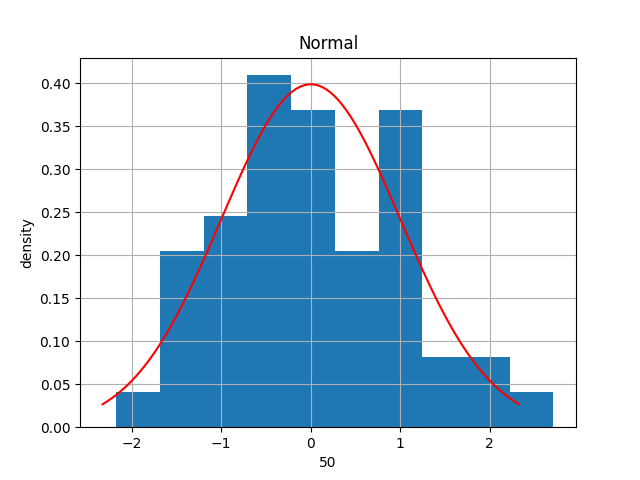
\includegraphics[height = 0.3\textheight, width = 0.3\textwidth]{Normal_size_50.png}
        & 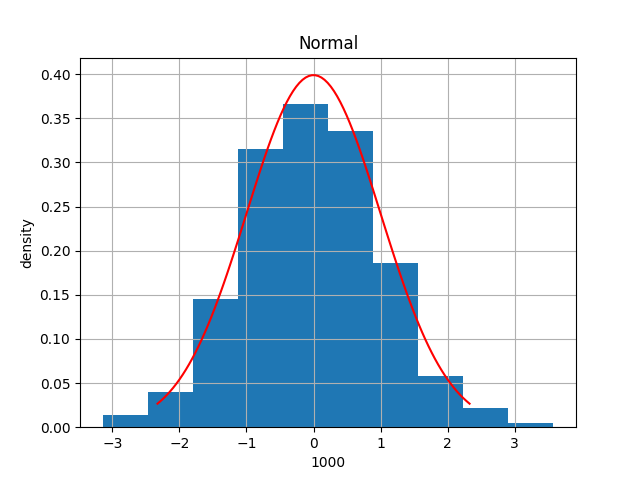
\includegraphics[height = 0.3\textheight, width = 0.3\textwidth]{Normal_size_1000.png}
    \end{tabular}
    \caption{Нормальное распределение}
    \label{fig:normal}
\end{figure}

\begin{figure}[H]
    \centering
    \begin{tabular}{c c c}
        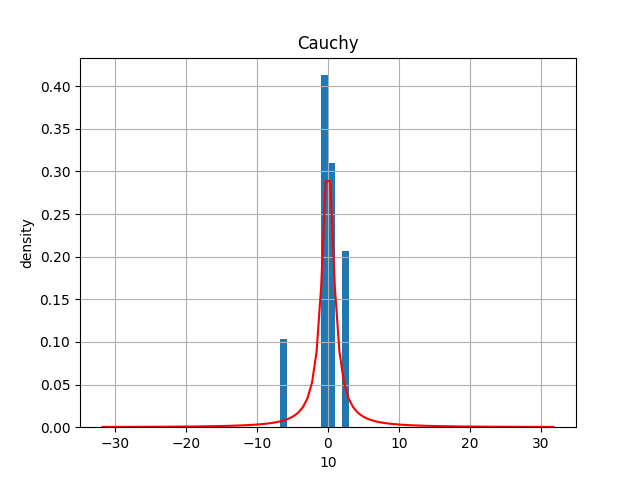
\includegraphics[height = 0.3\textheight, width = 0.3\textwidth]{Cauchy_size_10.png}
        & 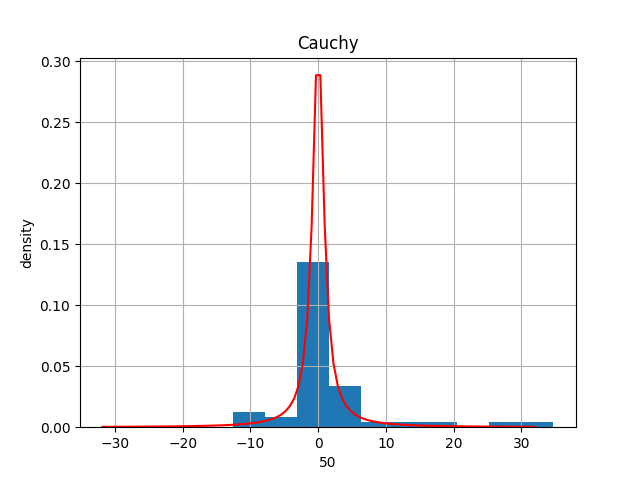
\includegraphics[height = 0.3\textheight, width = 0.3\textwidth]{Cauchy_size_50.png}
        & 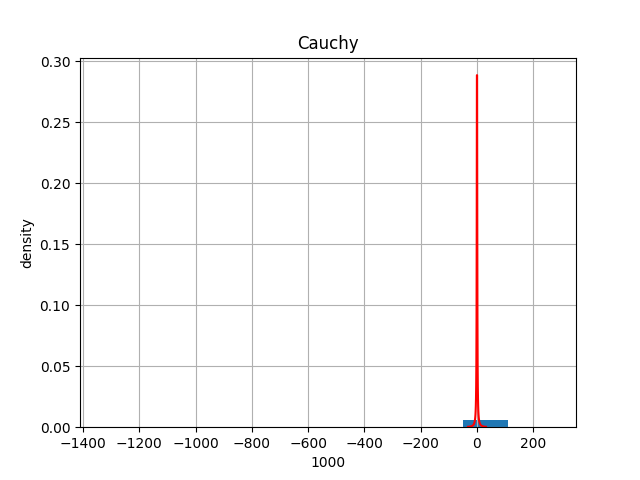
\includegraphics[height = 0.3\textheight, width = 0.3\textwidth]{Cauchy_size_1000.png}
    \end{tabular}
    \caption{Распределение Коши}
    \label{fig:cauchy}
\end{figure}

\begin{figure}[H]
    \centering
    \begin{tabular}{c c c}
        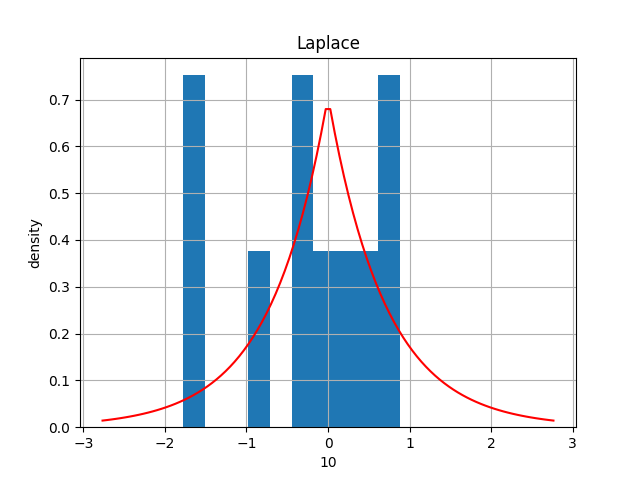
\includegraphics[height = 0.3\textheight, width = 0.3\textwidth]{Laplace_size_10.png}
        & 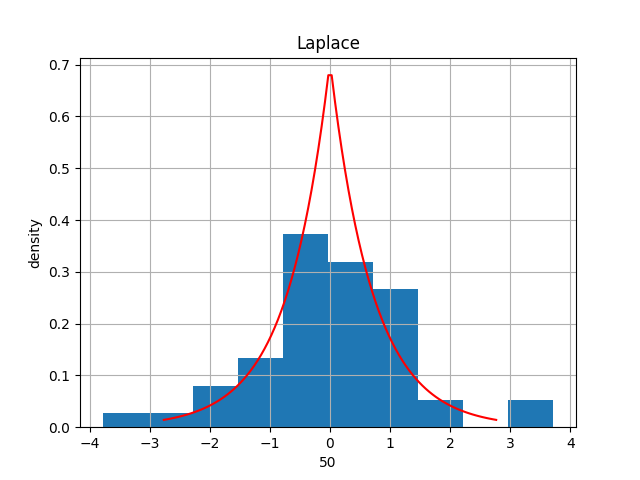
\includegraphics[height = 0.3\textheight, width = 0.3\textwidth]{Laplace_size_50.png}
        & 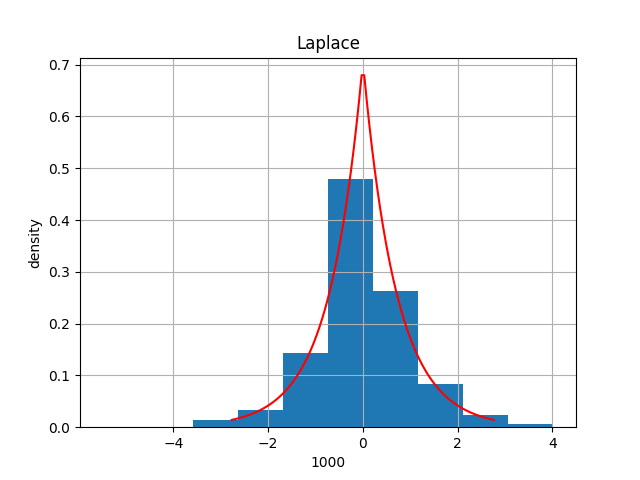
\includegraphics[height = 0.3\textheight, width = 0.3\textwidth]{Laplace_size_1000.png}
    \end{tabular}
    \caption{Распределение Лапласа}
    \label{fig:laplace}
\end{figure}

\begin{figure}[H]
    \centering
    \begin{tabular}{c c c}
        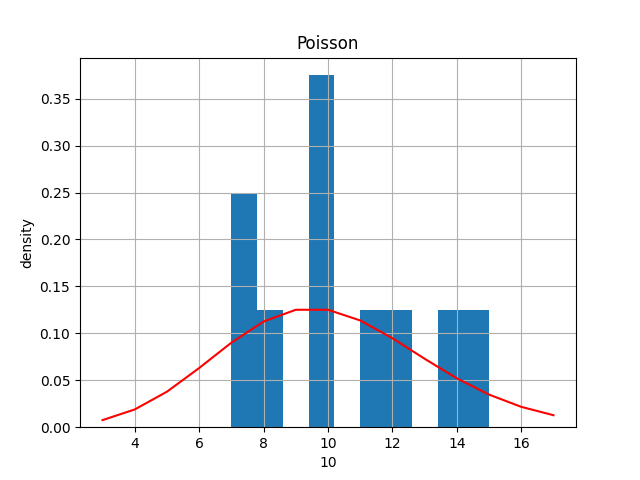
\includegraphics[height = 0.3\textheight, width = 0.3\textwidth]{Poisson_size_10.png}
        & 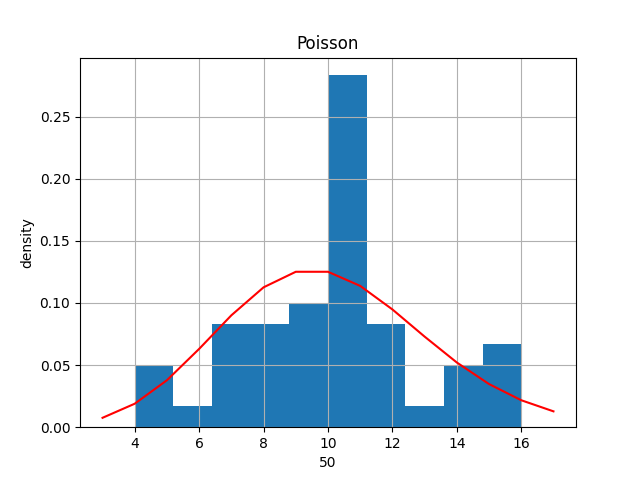
\includegraphics[height = 0.3\textheight, width = 0.3\textwidth]{Poisson_size_50.png}
        & 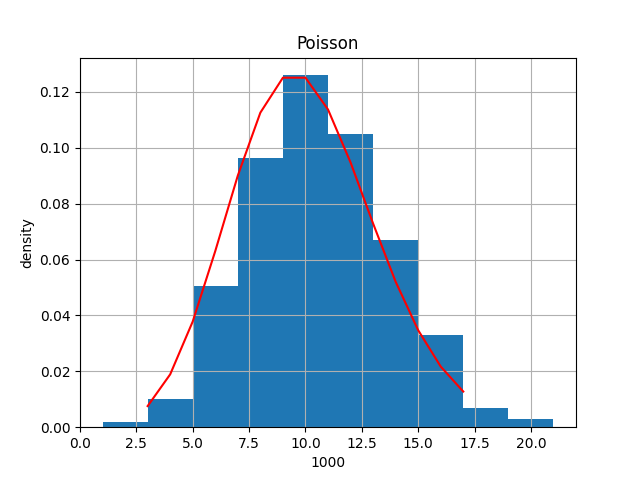
\includegraphics[height = 0.3\textheight, width = 0.3\textwidth]{Poisson_size_1000.png}
    \end{tabular}
    \caption{Распределение Пуассона}
    \label{fig:poisson}
\end{figure}

\begin{figure}[H]
    \centering
    \begin{tabular}{c c c}
        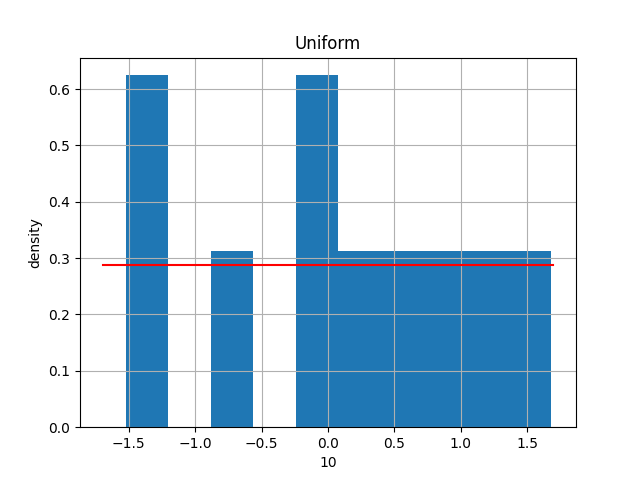
\includegraphics[height = 0.3\textheight, width = 0.3\textwidth]{Uniform_size_10.png}
        & 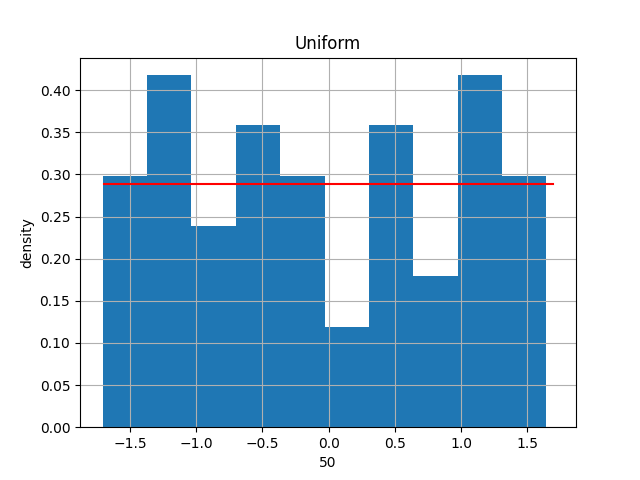
\includegraphics[height = 0.3\textheight, width = 0.3\textwidth]{Uniform_size_50.png}
        & 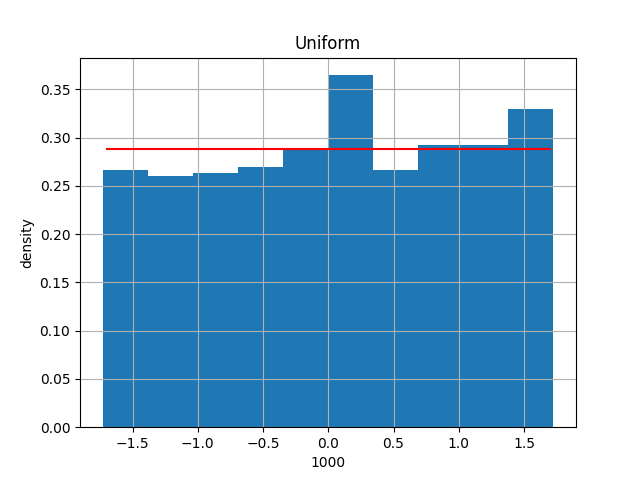
\includegraphics[height = 0.3\textheight, width = 0.3\textwidth]{Uniform_size_1000.png}
    \end{tabular}
    \caption{Равномерное распределение}
    \label{fig:uniform}
\end{figure}

\section{Обсуждение}
По полученным результатам видно, что увеличение выборки из распределения приближает гистограмму к графику плотности. Таким образом, рассмотрение выборки из большего числа элементов является более выгодным.

Также формы гистограмм, особенно для маленьких выборок, очень похожи друг над друга. Это объясняется тем, что чем меньше выборка. тем меньше гистограмма похожа на график плотности, и имеет более общий вид. В меньшей мере это касается распрделения Пуассона и равномерного, они имеют более широкий вид даже на маленьких выборках. А распределение Коши в свою очередь имеет более узкую форму, на большой выборке оно сходится к одному вертикальному столбцу. Однако, нормальное распределение и распределение Лапласа визуально почти неотличимы.

Всплески на гистограммах относительно плотности распредления также утихают по мере увеличения выборки. 

\end{document}